\documentclass[border=10pt]{standalone}
\usepackage{tikz}\usepackage{amsmath}\usetikzlibrary{arrows.meta}
\begin{document}
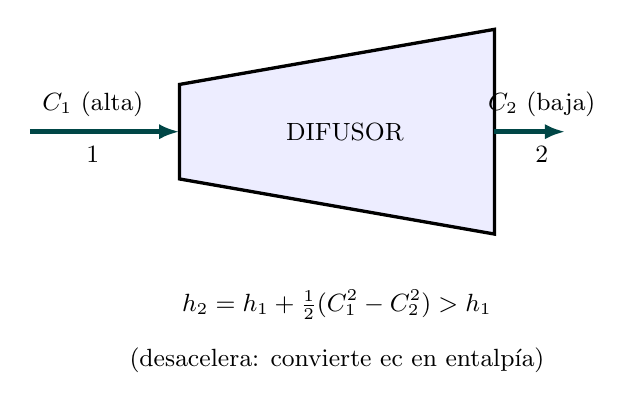
\begin{tikzpicture}[line width=1pt,>={Latex[length=2.6mm]}]
  \fill[blue!7] (0,0.9)--(0,2.1)--(4,2.8)--(4,0.2)--cycle;
  \draw[line width=1.2pt] (0,0.9)--(0,2.1)--(4,2.8)--(4,0.2)--cycle;
  \node at (2.1,1.5){\small DIFUSOR};
  % entrada rápida (flecha larga)
  \draw[->,teal!55!black,line width=1.6pt] (-1.9,1.5)--(0,1.5);
  \node[above] at (-1.1,1.55){\small $C_1$ (alta)}; \node[below] at (-1.1,1.45){\small $1$};
  % salida lenta (flecha corta)
  \draw[->,teal!55!black,line width=1.6pt] (4,1.5)--(4.9,1.5);
  \node[above] at (4.6,1.55){\small $C_2$ (baja)}; \node[below] at (4.6,1.45){\small $2$};
  \node at (2,-0.7){\small $h_2 = h_1 + \tfrac{1}{2}(C_1^2-C_2^2) > h_1$};
  \node at (2,-1.4){\small (desacelera: convierte ec en entalpía)};
\end{tikzpicture}
\end{document}
